\section{Variational Inference}
\subsection{Introduction to Variational Inference}
\textbf{variational inference} is an inference method which can help us to approximate a tractable inference. "Variational" refers to the technique in which complex probability distributions are approximated using simpler, parameterized distributions by optimizing over the parameters. We already see a similar application in rejection sampling, where $q(x)$ is the simpler distribution and help us to estimate the desired distribution, $p(x)$.
\subsubsection*{The posterior distribution of latent variable models}
Recall the joint distribution $p(x,z)=p(x)p(x|z)$. $x$ are the observed data points, $z$ are the unobserved (latent) data points. Moreover:
$$\underbrace{p(z|x)}_{\text{posterior}}=\frac{\overbrace{p(x|z)}^{\text{likelihood}}\overbrace{p(z)}^{\text{prior}}}{\underbrace{p(x)}_{\text{normalizing factor}}}$$
\begin{example}
    The TrueSkill model we introduced earlier is indeed a latent variable model.
    \begin{figure}[H]
        \centering
        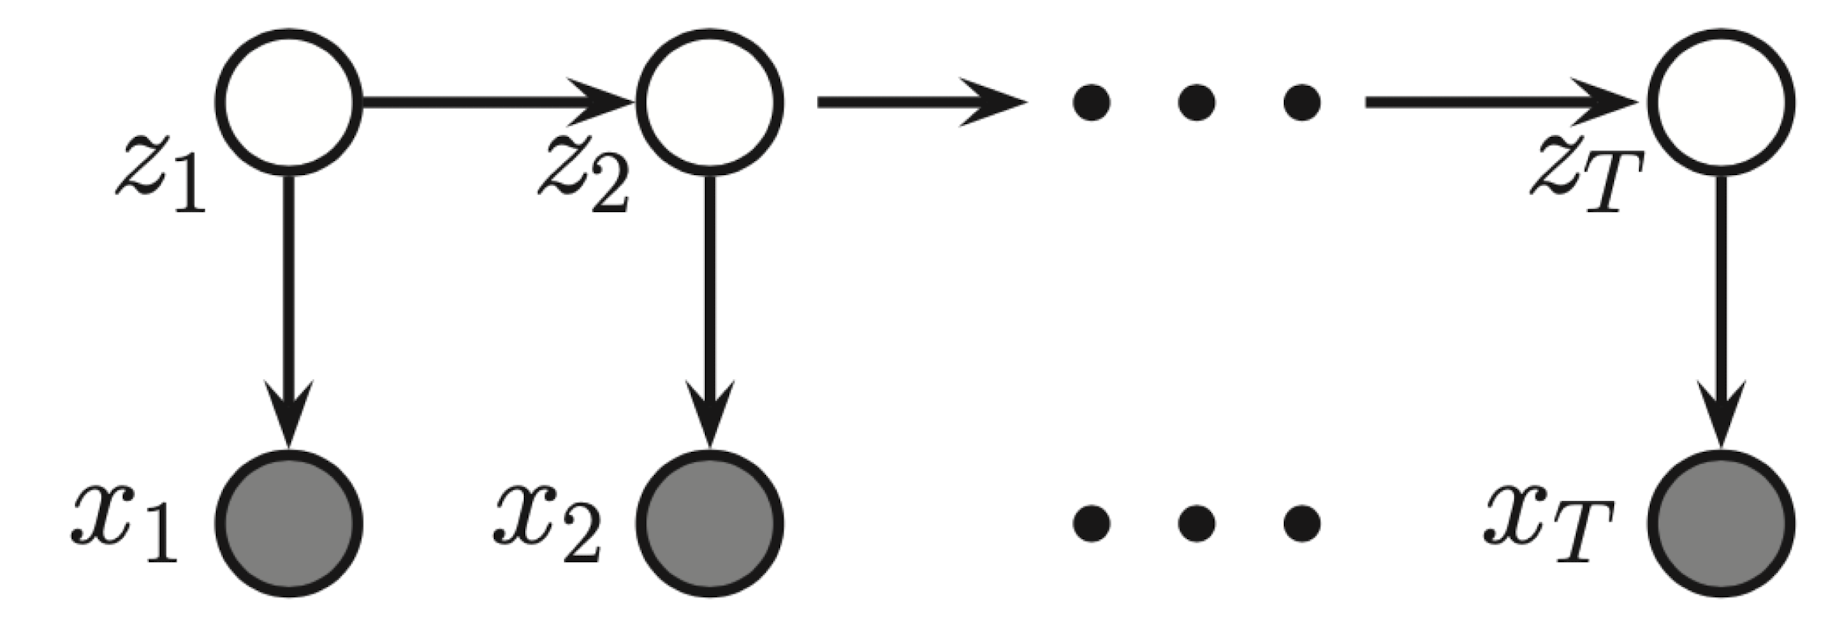
\includegraphics[width = .4\linewidth]{figures/section7/figure_7_1.png}
        \caption{Contour plot between two players}
        \label{fig:prior_trueskill}
    \end{figure}
    The above graph shows the contour graph between the two players. Since we assume both players follows Gaussian distribution, we are uncertain about players skills and hence we observe perfect "circles." Each contour represent different values of pdf. It goes higher when we move to the center. The blue dashed line represent equal skills between the two players. \href{https://en.wikipedia.org/wiki/Multivariate_normal_distribution#/media/File:Multivariate_Gaussian.png}{Here} is 3D view of the bivariate Gaussian distribution.
    \begin{figure}[H]
        \centering
        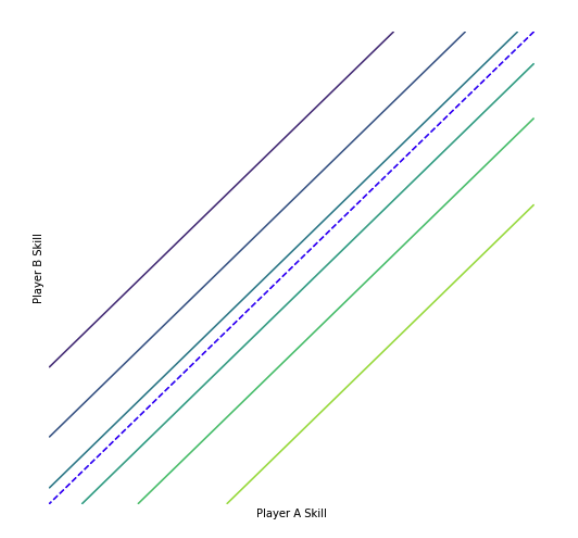
\includegraphics[width = .4\linewidth]{figures/section7/figure_7_2.png}
        \caption{2D projection of likelihood}
        \label{fig:likelihood_trueskill}
    \end{figure}
    The above graph shows the 2D projection of the likelihood $p(i\:\text{i beats j}|z_i,z_j)=\sigma(z_i-z_j)$.
    \begin{figure}[H]
        \centering
        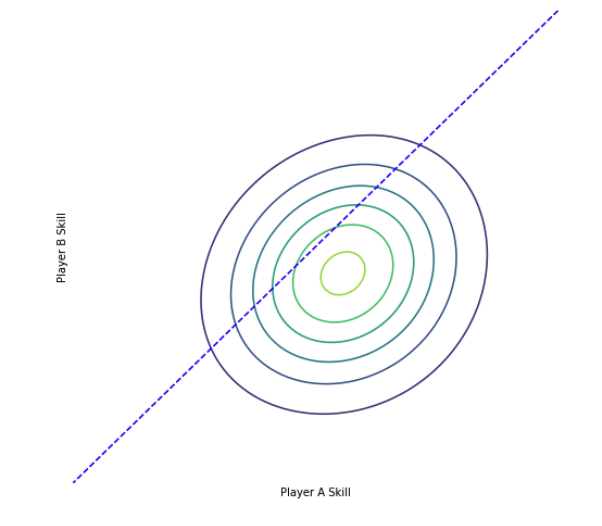
\includegraphics[width = .4\linewidth]{figures/section7/figure_7_3.png}
        \caption{The posterior}
        \label{fig:posterior_trueskill}
    \end{figure}
    The contours are not perfect "circles" anymore, which are not Gaussian anymore. However, the center moves to the left and we conclude that the guess player A is better than B.
\end{example}
\subsection{Kullback-Leibler divergence}
From the TrueSkill model, the normalizing factor $p(x)=\int p(x,z)dz$ is intractable when $z$ is high-dimensional. To estimate $p(x)$, like previously explained, our procedure is to approximate it using a simpler distribution $q(x)$. We measure the closeness/similarity between $p$ and $q$ using \textbf{KL Divergence}.
$$\mathrm{KL}(q(z) \| p(z \mid x))=\int q(z) \log \frac{q(z)}{p(z \mid x)} d z=\underset{z \sim q}{\mathbb{E}} \log \frac{q(z)}{p(z \mid x)}$$